\begin{figure}[htbp]
    \centering
    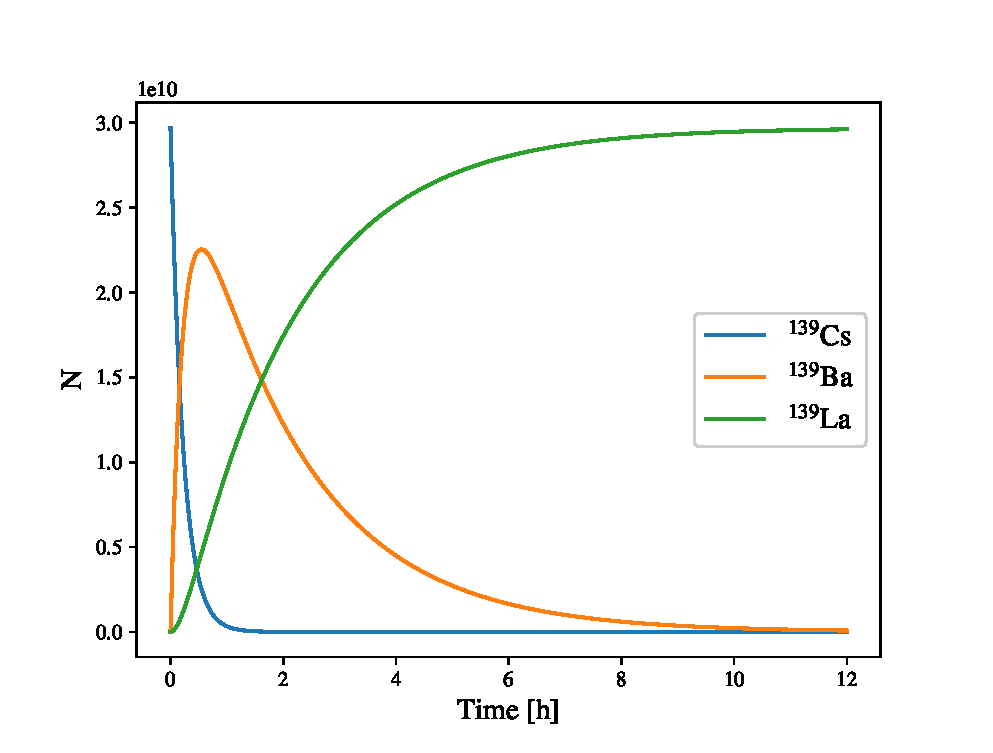
\includegraphics[scale=0.8]{ex7/decay.eps}
    \caption{Radioactive decay chain}
    \label{fig:decay_chain}
\end{figure}

\subsection*{a}
Said $N(t)$ the number of atoms present at time $t$, the radioactive decay law states that
\begin{equation}
    \mathcal{A} = -\frac{dN}{dt} = \lambda N
    \label{eq:decay_law}
\end{equation}
where $\lambda$ is called the decay constant. \\
By integrating it in time one obtains 
\begin{equation}
    N(t) = N_0 \, e^{-\lambda t}
    \label{eq:decay_chain_first_atom}
\end{equation}
Now if we consider a chain decay of the type $A \rightarrow B \rightarrow C$ with initial conditions 
\begin{equation*}
    N_A(t=0) = N_0 \qquad N_B(t=0) = N_C(t=0) = 0
\end{equation*}
one can immediately obtain the number of $A$ atoms as a function of time by applying \ref{eq:decay_law}
\begin{equation*}
    N_A(t) = N_0 e^{-\lambda_A t}
\end{equation*}
To study the number of atoms of type $B$ one has to take account of two factors: the number of "created" atoms by means of $A$'s decay, and
the number of atoms decayed into $C$. This means that the radioactive law reads 
\begin{equation*}
    N_B(t) = -\frac{1}{\lambda_B}\frac{dN_B(t)}{dt} + N_{A \to B}(t)
\end{equation*}
where the first term takes account of the fact on the right side member represents the $B$'s decay and the the last term 
represents the number of $B$ obtained by $A$'s decaying. \\
One can now substitute \ref{eq:decay_chain_first_atom} obtaining 
\begin{equation*}
    \frac{dN_B(t)}{dt} + \lambda_B N_B(t) =  N_0 \, e^{-\lambda_A t}
\end{equation*}
The general solution of this differential equation is 
\begin{equation*}
    N_B(t) = e^{-A(t)} \ \left(N_B(0) + \int_0^t N_0 e^{-\lambda_A s} e^{A(s)} \, ds \right)
\end{equation*}
where $A(s) = \lambda_B \int dt = \lambda_B t$. Hence
\begin{gather*}
N_B(t) = e^{-\lambda_B t} \ \int_0^t N_0 e^{-(\lambda_A - \lambda_B) s} \, ds 
= \frac{N_0 \, e^{-\lambda_B t}}{\lambda_A - \lambda_B} \ \left(1 - e^{-(\lambda_A - \lambda_B) t}\right) = \\
= N_0 \, \frac{e^{-\lambda_A t} - e^{-\lambda_B t}}{\lambda_B - \lambda_A}
\end{gather*}

\lstinputlisting[language=python, showstringspaces=false]{ex7/ex7.py}